% Reporte de métricas: contención de CPU y memoria, MongoDB vs PostgreSQL JSONB.
% Compilar desde esta carpeta:  latexmk -pdf reporte.tex
% Las tablas y figuras de generado/ salen de analysis/consolidar.py (no se editan a mano).
\documentclass[11pt,a4paper]{article}
\usepackage[spanish,es-noshorthands,es-tabla]{babel}
\usepackage[T1]{fontenc}
\usepackage{lmodern}
\usepackage[margin=2.2cm]{geometry}
\usepackage{booktabs,longtable,array,multirow}
\usepackage{graphicx}
\usepackage{xcolor}
\usepackage{listings}
\usepackage{caption}
\usepackage{enumitem}
\usepackage[hidelinks]{hyperref}

\captionsetup{font=small,labelfont=bf}
\setlength{\emergencystretch}{3em}
\setlist{itemsep=2pt,topsep=4pt}
\lstset{basicstyle=\ttfamily\footnotesize,breaklines=true,columns=fullflexible,
  frame=single,rulecolor=\color{black!25},xleftmargin=2pt,xrightmargin=2pt,
  literate={á}{{\'a}}1 {é}{{\'e}}1 {í}{{\'i}}1 {ó}{{\'o}}1 {ú}{{\'u}}1 {ñ}{{\~n}}1 {×}{{$\times$}}1}
\newcommand{\cod}[1]{\texttt{#1}}

\title{Contención de CPU y memoria en bases de datos documentales:\\
MongoDB frente a PostgreSQL JSONB con límites de Docker (cgroups v2)\\[4pt]
\large Reporte de métricas}
\author{Ángel Eduardo Chamé Pérez \\[2pt]
\small Bases de Datos en la Nube \\
\small Universidad Politécnica de Chiapas (IT2iD) \\
\small Grupo 7-B \\
\small Profesor: Horacio Irán Solís Cisneros}
\date{1 de noviembre de 2026}

\begin{document}
\maketitle

\begin{abstract}
\noindent Se midió el comportamiento de MongoDB 9.0.4 y PostgreSQL 18.6 (JSONB) con
500\,000 ventas sintéticas de un sistema de abarrotes, bajo tres perfiles de límites de
Docker (4 CPU/4 GiB, 2 CPU/2 GiB y 1 CPU/1 GiB), dos consultas (Q1, agregación con
desanidado, orientada a CPU; Q2, filtro con ordenamiento Top-1000, orientada a memoria) y
1, 10 y 50 clientes concurrentes. La matriz de 38 celdas se repitió en 3 rondas
(114 corridas de 300\,s, sin descartes): 87 corridas terminaron \cod{ok}, 21 con
volcado a disco (\cod{spill}) y 6 con \cod{oom}. Todas las corridas \cod{spill} y
\cod{oom} son de PostgreSQL con Q1: su plan ordena los documentos completos antes de
agrupar y escribe unos 0,8\,GiB de archivos temporales por ejecución, su P99 es entre
2,0 y 13,6 veces el de MongoDB en las celdas que terminan sin OOM, y con 50 clientes
agota la memoria en los perfiles B y C. En Q2 ambos motores escalan en proporción a la
cuota de CPU; PostgreSQL es más rápido con 1 cliente y logra unas 1,3 veces más
QPS con 50 clientes, y ninguna de las variantes de memoria de Q2 vuelca a disco. Por cada
1\,000 documentos procesados (definición adoptada en este reporte; el enunciado no la
precisa), Q1 con 1 cliente usa 8,7--11,8\,ms de
CPU en PostgreSQL frente a 2,9--3,2\,ms en MongoDB, y Q2 entre 1,1 y 1,8\,ms en ambos.
\end{abstract}

\tableofcontents
\clearpage

%=====================================================================
\section{Especificaciones del host y del entorno Docker}
%=====================================================================
% P-24: fuente de la aceptación pendiente
Las mediciones se hicieron con Docker Desktop sobre WSL2 en Windows, no en Linux nativo
(ver ``Desviaciones y limitaciones''). La captura completa del entorno está en
\cod{evidence/entorno/} (\cod{entorno.json} y salidas crudas).

\begin{table}[h]
\centering\small
\caption{Host y entorno de ejecución}\label{tab:host}
\begin{tabular}{@{}p{0.27\linewidth}p{0.68\linewidth}@{}}
\toprule
Equipo & HP Victus 15-fb2xxx (laptop), conectada a la corriente durante toda la matriz \\
CPU & AMD Ryzen 5 8645HS, 6 núcleos / 12 hilos, hasta 4,3\,GHz \\
RAM del host & 15,3\,GiB \\
Disco & SSD NVMe WD PC SN560, 1\,TB \\
Sistema & Windows 11 Home Single Language 10.0.26200 (64 bits); modo de energía
  ``máximo rendimiento'' con corriente alterna \\
WSL & 2.6.3.0; kernel \cod{6.6.87.2-microsoft-standard-WSL2}; sin \cod{.wslconfig}
  (valores por defecto) \\
Máquina virtual de Docker & 12 CPU, 7,39\,GiB de RAM, 2\,GiB de swap de la VM \\
Docker & Docker Desktop 4.97.0, Engine 29.9.2, Compose 5.6.1; cgroups v2 (driver
  \cod{cgroupfs}); almacenamiento \cod{overlayfs} \\
Cliente de carga & Python 3.12.10 en Windows (fuera de la VM); pymongo 4.19.0,
  psycopg 3.3.6 \\
\bottomrule
\end{tabular}
\end{table}

\begin{table}[h]
\centering\small
\caption{Imágenes usadas (etiqueta exacta y digest) y versión que reporta cada motor}\label{tab:imagenes}
\begin{tabular}{@{}lll@{}}
\toprule
Imagen & Versión que reporta & Digest \\
\midrule
\cod{mongo:9.0.4} & 9.0.4 & (1) \\
\cod{postgres:18.6} & 18.6 (Debian 18.6-1.pgdg13+2) & (2) \\
\cod{prom/prometheus:v3.15.1} & --- & (3) \\
\cod{prom/node-exporter:v1.12.1} & --- & (4) \\
\cod{ghcr.io/google/cadvisor:v0.60.6} & --- & (5) \\
\bottomrule
\end{tabular}

\smallskip
{\scriptsize\ttfamily
\begin{tabular}{@{}ll@{}}
(1) & sha256:452bdaf2127b8ff851e31410a267809b9829eded219979f2210e7c7efb85a058 \\
(2) & sha256:3a4264520e121176619f54ff867d12774bc81e95e7b84db58d63bccdb6144b81 \\
(3) & sha256:fa3302279710be2f21a8301ec17a8b4f2301fd829bd113839b3b6b02b6f191a2 \\
(4) & sha256:1b4e4438faca4dd7e001dd445d161a4a2091b0fededa84093b3a8dfeae1f1be0 \\
(5) & sha256:b8e7d1093144fd088f425ff003d75a4aa405de075db78dae3bc563730b1bd07a \\
\end{tabular}}
\end{table}

\paragraph{Perfiles de recursos.} Cada motor corre solo (el otro contenedor está
apagado) y se recrea en cada corrida con los límites del perfil. Los límites se
verificaron leyendo el cgroup real del contenedor
(\cod{evidence/verificacion/limites.json}) y se vuelven a leer y guardar en cada
corrida (\cod{meta.json}, campo \cod{identidad.limites}).

\begin{table}[h]
\centering\small
\caption{Perfiles y límites reales leídos del cgroup}\label{tab:perfiles}
\begin{tabular}{@{}lccccc@{}}
\toprule
Perfil & \cod{cpus} & \cod{mem\_limit} & \cod{cpu.max} & \cod{memory.max} & \cod{memory.swap.max} \\
\midrule
A (\cod{PROFILE\_A\_BASELINE}) & 4 & 4096\,MiB & \cod{400000 100000} & 4\,294\,967\,296 & 0 \\
B (\cod{PROFILE\_B\_MEDIUM})   & 2 & 2048\,MiB & \cod{200000 100000} & 2\,147\,483\,648 & 0 \\
C (\cod{PROFILE\_C\_SEVERE})   & 1 & 1024\,MiB & \cod{100000 100000} & 1\,073\,741\,824 & 0 \\
\bottomrule
\end{tabular}
\end{table}

\noindent Configuración de los motores: la de cada imagen, sin ajustes de memoria ni de
paralelismo. MongoDB se publica en el puerto 27018 del host (el 27017 lo ocupa otro
servicio, detenido durante toda la matriz). PostgreSQL usa la base \cod{benchmark} con
collation C y \cod{shm\_size: 1g} (desviación declarada). La telemetría la recogen
cAdvisor y Node Exporter, consultados por Prometheus cada segundo.

%=====================================================================
\section{Método de medición y verificación del baseline}
%=====================================================================
\subsection{Datos y consultas}
El documento es una venta del sistema de abarrotes del autor (datos sintéticos): folio,
fecha ISO-8601 UTC, tipo de pago (\cod{EFECTIVO}, \cod{TRANSFERENCIA}, \cod{FIADO}),
total, bandera \cod{es\_fiado} y una lista \cod{items} de 1 a 10 artículos (promedio 3,0);
cada artículo lleva \cod{producto.proveedor.\{id, empresa\}}, lo que da 4 niveles de
anidamiento. Se generaron 500\,000 ventas con semilla fija (20261101) en un solo archivo
NDJSON (SHA-256 \cod{59c35b36\ldots2ad6a8c1}, 940,2\,B por venta) que se cargó en ambos
motores: colección \cod{ventas} en MongoDB y tabla \cod{ventas(id UUID PRIMARY KEY,
data JSONB)} en PostgreSQL. Índices: en MongoDB, \cod{fecha} y \cod{folio}; en
PostgreSQL, la llave primaria y un B-Tree sobre \cod{(data->>'fecha')}.

\begin{lstlisting}[caption={Q1 (CPU): desanidar, filtrar, calcular y agrupar}]
-- PostgreSQL
SELECT data->>'tipo_pago', item->'producto'->'proveedor'->>'id',
       SUM((item->>'cantidad')::numeric * (item->>'precio_unitario')::numeric),
       AVG((item->>'cantidad')::numeric * (item->>'precio_unitario')::numeric)
FROM ventas, jsonb_array_elements(data->'items') AS item
WHERE (item->>'precio_unitario')::numeric > 50
GROUP BY 1, 2
// MongoDB
[{$unwind: "$items"}, {$match: {"items.precio_unitario": {$gt: 50}}},
 {$project: {tipo_pago: 1, proveedor_id: "$items.producto.proveedor.id",
             subtotal: {$multiply: ["$items.cantidad", "$items.precio_unitario"]}}},
 {$group: {_id: {tipo_pago: "$tipo_pago", proveedor_id: "$proveedor_id"},
           suma_subtotal: {$sum: "$subtotal"}, promedio_subtotal: {$avg: "$subtotal"}}}]
\end{lstlisting}

\begin{lstlisting}[caption={Q2 (memoria): filtrar y ordenar sin índice, Top-1000}]
-- PostgreSQL (Q2: SET work_mem = '4MB'; Q2_RELAXED: SET work_mem = '64MB')
SELECT data FROM ventas
WHERE (data->>'es_fiado')::boolean = false AND data->>'fecha' >= '2026-01-01T00:00:00Z'
ORDER BY (data->>'total')::numeric DESC, (data->>'folio')::int ASC
LIMIT 1000
// MongoDB (Q2: allowDiskUse false; Q2_RELAXED: allowDiskUse true)
[{$match: {es_fiado: false, fecha: {$gte: "2026-01-01T00:00:00Z"}}},
 {$sort: {total: -1, folio: 1}}, {$limit: 1000}]
\end{lstlisting}

\subsection{Matriz y protocolo}
La matriz tiene 38 celdas: 2 motores $\times$ 3 perfiles $\times$ 2 consultas (Q1, Q2)
$\times$ 3 concurrencias (1, 10, 50), más \cod{Q2\_RELAXED} con 50 clientes en el
perfil C para cada motor. Se ejecutó en 3 rondas completas; dentro de cada ronda el orden
de las celdas es aleatorio con semilla fija (\cod{random.Random("20261101:ronda:<n>")}),
para que la hora del día no se confunda con el perfil. El número de ronda es el
\cod{run\_number} del CSV. Cada corrida sigue estos pasos (\cod{runner/run\_cell.py}):
\begin{enumerate}
\item Precondiciones: laptop conectada, servicio MongoDB de Windows detenido y al menos
  60\,GB libres en disco.
\item Recrear el contenedor del motor con los límites del perfil (el otro motor queda
  apagado) y verificar su identidad: puerto, versión exacta, un dato propio del
  contenedor (hostname o IP) y los límites del cgroup. Si no coinciden, la corrida aborta.
\item Vaciar la caché de páginas de la VM (\cod{drop\_caches}).
\item Lanzar $c$ procesos cliente (\cod{multiprocessing}, modo \cod{spawn}), cada uno con
  su propia conexión, en lazo cerrado y sin pausa entre consultas.
\item 60\,s de calentamiento, 300\,s de medición y 60\,s de enfriamiento. Timeout por
  consulta: 300\,s. Las consultas que siguen en curso al cerrar la ventana se cancelan y
  no se cuentan.
\end{enumerate}

\subsection{Métricas}
\begin{itemize}
\item \textbf{Throughput (QPS):} consultas exitosas que empezaron y terminaron dentro de
  la ventana, entre 300\,s.
\item \textbf{Latencias P50/P95/P99:} percentil por rango más cercano sobre las
  latencias de esas consultas. Con menos de 100 consultas el P99 coincide con el máximo y
  así se rotula; entre 100 y 999, el P99 se considera orientativo.
\item \textbf{Throttling de CPU:} diferencia de \cod{throttled\_usec} de
  \cod{cpu.stat} del cgroup entre el inicio y el fin de la ventana. En cgroups v2 este
  contador acumula el tiempo de espera de todas las CPU en que el grupo tenía hilos
  listos, por lo que puede superar los 300\,s de reloj. Se complementa con la fracción de
  periodos CFS con throttling (\cod{nr\_throttled}/\cod{nr\_periods}).
\item \textbf{RSS máxima:} máximo de \cod{container\_memory\_rss} de cAdvisor en la
  ventana; también se guarda \cod{memory.peak} del cgroup, que incluye caché de página.
\item \textbf{Volcado a disco:} bytes temporales en la ventana: \cod{temp\_bytes} de
  \cod{pg\_stat\_database} en PostgreSQL; \cod{spillToDiskBytes} y
  \cod{spilledDataStorageSize} de \cod{serverStatus} en MongoDB.
\item \textbf{OOM:} \cod{oom\_kill} de \cod{memory.events} y la bandera
  \cod{OOMKilled} de Docker.
\item \textbf{Estado:} prioridad \cod{oom} $>$ \cod{error} $>$ \cod{spill} $>$
  \cod{ok}. Una corrida se descarta solo por una causa externa fijada de antemano
  (corriente, suspensión, caída de Docker); un OOM o un volcado son resultados, no
  descartes.
\end{itemize}
Cada corrida deja \cod{meta.json} (identidad, contadores del cgroup, consultas, temporales),
\cod{latencias.csv} (todas las consultas), \cod{serie\_1s.csv} (RSS y throttling cada
segundo) y, si hubo \cod{oom} o \cod{error}, \cod{docker\_logs.txt}.

\subsection{Verificación del baseline}
Antes del piloto se comprobó que ambos motores tienen los mismos datos y devuelven lo
mismo (\cod{runner/verificar\_f2.py}; detalle en \cod{evidence/verificacion/}). Todas las
condiciones se cumplieron:
\begin{itemize}
\item 500\,000 ventas en cada motor; 1\,998 documentos de muestra idénticos entre motores.
\item Tamaño por venta: 940,2\,B en JSON, 984\,B en BSON y 1\,174,6\,B en JSONB.
\item Q1: los mismos 90 grupos y 674\,686 artículos; diferencia máxima de las sumas
  $9{,}3\times10^{-10}$ (tolerancia: 1 centavo).
\item Q2 y \cod{Q2\_RELAXED}: las mismas 1\,000 filas en el mismo orden en ambos motores.
\item Con 1 cliente en el perfil A, Q1 tarda 2,06\,s en MongoDB y 3,44\,s en PostgreSQL;
  Q2, 0,28\,s y 0,25\,s (una sola ejecución, no es medición).
\item Los límites reales de los 6 contenedores coinciden con su perfil y
  \cod{drop\_caches} funciona en la VM (caché de 850\,MB a 375\,MB).
\end{itemize}

\subsection{Ejecución}
Un piloto de 3 corridas (resultados en \cod{results/piloto/}, fuera de la matriz) fijó
la duración real: unos 7,4\,min por corrida. La matriz se lanzó el 1 de noviembre de
2026 a las 01:15 (hora de la Ciudad de México) y terminó a las 16:09. Según
\cod{results/bitacora.log}, hubo una sola pausa, entre corridas, de 11:59 a 12:49; al
reanudar, el orquestador volvió a revisar el entorno. Las 114 corridas tienen fila en el
CSV, sin descartes ni reintentos. Al cerrar cada ronda se hizo un respaldo con manifiesto
SHA-256, verificado con \cod{sha256sum -c}.

%=====================================================================
\section{Resultados consolidados}
%=====================================================================
Las tablas~\ref{tab:rendimiento} y~\ref{tab:recursos} resumen cada celda con la mediana
de sus 3 rondas y el rango del P99 entre rondas. Se usa la mediana y no la media porque
con 3 valores no se deja arrastrar por una ronda atípica. Las 114 filas individuales están
en \cod{results/benchmark\_results.csv}; el resumen por celda, en
\cod{report/generado/celdas.csv}.

\paragraph{Estados.} Las tres rondas dan exactamente los mismos estados: por ronda,
29 corridas \cod{ok}, 7 \cod{spill} y 2 \cod{oom}, sin \cod{error}. Todas las corridas
\cod{spill} y \cod{oom} son de PostgreSQL con Q1; MongoDB no tuvo volcado a disco ni OOM
en ninguna celda.

{\small\setlength{\tabcolsep}{3.5pt}
\begin{longtable}{llcrlrrrrr}
\caption{Rendimiento por celda (ventana de 300 s)}\label{tab:rendimiento}\\
\toprule
 & Motor & Perfil & $c$ & Estados & QPS & \begin{tabular}[b]{@{}c@{}}P50\\(ms)\end{tabular} & \begin{tabular}[b]{@{}c@{}}P95\\(ms)\end{tabular} & \begin{tabular}[b]{@{}c@{}}P99\\(ms)\end{tabular} & \begin{tabular}[b]{@{}c@{}}P99 entre rondas\\mín.--máx. (ms)\end{tabular} \\
\midrule
\endfirsthead
\toprule
 & Motor & Perfil & $c$ & Estados & QPS & \begin{tabular}[b]{@{}c@{}}P50\\(ms)\end{tabular} & \begin{tabular}[b]{@{}c@{}}P95\\(ms)\end{tabular} & \begin{tabular}[b]{@{}c@{}}P99\\(ms)\end{tabular} & \begin{tabular}[b]{@{}c@{}}P99 entre rondas\\mín.--máx. (ms)\end{tabular} \\
\midrule
\endhead
\midrule
\multicolumn{10}{r}{\footnotesize continúa}\\
\endfoot
\bottomrule
\multicolumn{10}{p{0.95\linewidth}}{\footnotesize Q2R: \texttt{Q2\_RELAXED}. Mediana de las 3 rondas por celda; P99 mín.--máx. entre rondas. Percentiles por rango más cercano sobre las consultas exitosas de la ventana (D-007): $^{\dagger}$ menos de 100 consultas en alguna ronda, el P99 es igual al máximo; $^{\ddagger}$ entre 100 y 999, P99 orientativo. ``---'': sin consultas terminadas.}\\
\endlastfoot
Q1 & MongoDB & A & 1 & 3$\times$ok & 0{,}77 & 1\,279 & 1\,359 & 1\,411$^{\ddagger}$ & 1\,356--1\,435 \\
Q1 & MongoDB & A & 10 & 3$\times$ok & 1{,}72 & 5\,708 & 5\,923 & 6\,090$^{\ddagger}$ & 5\,806--6\,396 \\
Q1 & MongoDB & A & 50 & 3$\times$ok & 1{,}48 & 30\,704 & 33\,419 & 35\,077$^{\ddagger}$ & 34\,592--35\,198 \\
Q1 & MongoDB & B & 1 & 3$\times$ok & 0{,}76 & 1\,304 & 1\,387 & 1\,429$^{\ddagger}$ & 1\,419--1\,571 \\
Q1 & MongoDB & B & 10 & 3$\times$ok & 0{,}87 & 10\,995 & 11\,505 & 11\,808$^{\ddagger}$ & 11\,594--12\,393 \\
Q1 & MongoDB & B & 50 & 3$\times$ok & 0{,}67 & 58\,995 & 64\,498 & 66\,694$^{\ddagger}$ & 66\,497--67\,097 \\
Q1 & MongoDB & C & 1 & 3$\times$ok & 0{,}63 & 1\,461 & 2\,027 & 2\,063$^{\ddagger}$ & 1\,988--2\,148 \\
Q1 & MongoDB & C & 10 & 3$\times$ok & 0{,}42 & 22\,293 & 23\,801 & 24\,799$^{\ddagger}$ & 23\,503--25\,702 \\
Q1 & MongoDB & C & 50 & 3$\times$ok & 0{,}30 & 115\,995 & 127\,894 & 137\,694$^{\dagger}$ & 133\,193--138\,096 \\
\addlinespace
Q1 & PostgreSQL & A & 1 & 3$\times$spill & 0{,}37 & 2\,676 & 2\,744 & 2\,790$^{\ddagger}$ & 2\,758--2\,941 \\
Q1 & PostgreSQL & A & 10 & 3$\times$spill & 0{,}17 & 44\,561 & 80\,579 & 82\,581$^{\dagger}$ & 82\,456--86\,205 \\
Q1 & PostgreSQL & A & 50 & 3$\times$spill & 0{,}01 & 179\,946 & 210\,294 & 210\,294$^{\dagger}$ & 188\,248--211\,003 \\
Q1 & PostgreSQL & B & 1 & 3$\times$spill & 0{,}25 & 3\,822 & 5\,038 & 5\,343$^{\dagger}$ & 3\,283--5\,789 \\
Q1 & PostgreSQL & B & 10 & 3$\times$spill & 0{,}13 & 62\,638 & 74\,523 & 74\,662$^{\dagger}$ & 70\,775--77\,263 \\
Q1 & PostgreSQL & B & 50 & 3$\times$oom & 0{,}01 & 133\,112 & 157\,157 & 157\,157$^{\dagger}$ & 131\,864--176\,270 \\
Q1 & PostgreSQL & C & 1 & 3$\times$spill & 0{,}14 & 7\,290 & 8\,179 & 8\,497$^{\dagger}$ & 8\,233--11\,142 \\
Q1 & PostgreSQL & C & 10 & 3$\times$spill & 0{,}08 & 93\,100 & 104\,898 & 105\,002$^{\dagger}$ & 97\,429--110\,414 \\
Q1 & PostgreSQL & C & 50 & 3$\times$oom & 0{,}00 & --- & --- & --- & --- \\
\addlinespace
Q2 & MongoDB & A & 1 & 3$\times$ok & 4{,}09 & 243 & 257 & 270 & 269--278 \\
Q2 & MongoDB & A & 10 & 3$\times$ok & 10{,}70 & 908 & 1\,086 & 1\,108 & 1\,105--1\,116 \\
Q2 & MongoDB & A & 50 & 3$\times$ok & 9{,}74 & 5\,011 & 7\,517 & 8\,587 & 8\,516--8\,599 \\
Q2 & MongoDB & B & 1 & 3$\times$ok & 3{,}95 & 250 & 275 & 289 & 282--292 \\
Q2 & MongoDB & B & 10 & 3$\times$ok & 5{,}55 & 1\,794 & 2\,091 & 2\,193 & 2\,108--2\,415 \\
Q2 & MongoDB & B & 50 & 3$\times$ok & 5{,}09 & 9\,294 & 15\,498 & 18\,087 & 17\,705--18\,295 \\
Q2 & MongoDB & C & 1 & 3$\times$ok & 3{,}59 & 248 & 502 & 587 & 520--593 \\
Q2 & MongoDB & C & 10 & 3$\times$ok & 2{,}80 & 3\,499 & 4\,105 & 4\,503$^{\ddagger}$ & 4\,408--4\,506 \\
Q2 & MongoDB & C & 50 & 3$\times$ok & 2{,}59 & 17\,804 & 27\,504 & 31\,686$^{\ddagger}$ & 31\,498--35\,196 \\
\addlinespace
Q2 & PostgreSQL & A & 1 & 3$\times$ok & 6{,}65 & 149 & 163 & 175 & 175--177 \\
Q2 & PostgreSQL & A & 10 & 3$\times$ok & 10{,}22 & 896 & 1\,410 & 1\,524 & 1\,520--1\,579 \\
Q2 & PostgreSQL & A & 50 & 3$\times$ok & 12{,}93 & 3\,678 & 5\,523 & 6\,755 & 6\,719--6\,817 \\
Q2 & PostgreSQL & B & 1 & 3$\times$ok & 5{,}54 & 183 & 202 & 218 & 207--219 \\
Q2 & PostgreSQL & B & 10 & 3$\times$ok & 5{,}64 & 1\,597 & 2\,592 & 2\,792 & 2\,789--2\,916 \\
Q2 & PostgreSQL & B & 50 & 3$\times$ok & 6{,}68 & 6\,978 & 11\,117 & 12\,907 & 12\,805--12\,999 \\
Q2 & PostgreSQL & C & 1 & 3$\times$ok & 2{,}87 & 328 & 398 & 411$^{\ddagger}$ & 402--460 \\
Q2 & PostgreSQL & C & 10 & 3$\times$ok & 2{,}88 & 3\,084 & 5\,097 & 5\,703$^{\ddagger}$ & 5\,307--5\,714 \\
Q2 & PostgreSQL & C & 50 & 3$\times$ok & 3{,}42 & 12\,992 & 21\,732 & 25\,294$^{\ddagger}$ & 24\,796--26\,290 \\
\addlinespace
Q2R & MongoDB & C & 50 & 3$\times$ok & 2{,}62 & 17\,286 & 27\,297 & 31\,795$^{\ddagger}$ & 30\,406--34\,405 \\
\addlinespace
Q2R & PostgreSQL & C & 50 & 3$\times$ok & 3{,}45 & 12\,887 & 21\,610 & 25\,389 & 25\,097--25\,390 \\
\end{longtable}
}

{\small\setlength{\tabcolsep}{3.5pt}
\begin{longtable}{llcrrrrrrr}
\caption{Recursos por celda (ventana de 300 s)}\label{tab:recursos}\\
\toprule
 & Motor & Perfil & $c$ & \begin{tabular}[b]{@{}c@{}}Throttling\\(s)\end{tabular} & \begin{tabular}[b]{@{}c@{}}Periodos con\\throttling (\%)\end{tabular} & \begin{tabular}[b]{@{}c@{}}RSS máx.\\(MiB)\end{tabular} & \begin{tabular}[b]{@{}c@{}}Pico cgroup\\(MiB)\end{tabular} & \begin{tabular}[b]{@{}c@{}}Temporales\\(GiB)\end{tabular} & \begin{tabular}[b]{@{}c@{}}Consultas\\ok\end{tabular} \\
\midrule
\endfirsthead
\toprule
 & Motor & Perfil & $c$ & \begin{tabular}[b]{@{}c@{}}Throttling\\(s)\end{tabular} & \begin{tabular}[b]{@{}c@{}}Periodos con\\throttling (\%)\end{tabular} & \begin{tabular}[b]{@{}c@{}}RSS máx.\\(MiB)\end{tabular} & \begin{tabular}[b]{@{}c@{}}Pico cgroup\\(MiB)\end{tabular} & \begin{tabular}[b]{@{}c@{}}Temporales\\(GiB)\end{tabular} & \begin{tabular}[b]{@{}c@{}}Consultas\\ok\end{tabular} \\
\midrule
\endhead
\midrule
\multicolumn{10}{r}{\footnotesize continúa}\\
\endfoot
\bottomrule
\multicolumn{10}{p{0.95\linewidth}}{\footnotesize Q2R: \texttt{Q2\_RELAXED}. Mediana de las 3 rondas salvo RSS y pico del cgroup (máximo). Throttling: delta de \texttt{throttled\_usec} de \texttt{cpu.stat}, que suma el tiempo de todas las CPU del grupo y puede superar los 300 s de la ventana. Periodos con throttling: \texttt{nr\_throttled}/\texttt{nr\_periods}. RSS: cAdvisor (\texttt{container\_memory\_rss}); pico del cgroup: \texttt{memory.peak}, que incluye caché de página y memoria compartida desde el arranque del contenedor. Temporales: \texttt{pg\_stat\_database.temp\_bytes} (PostgreSQL) o \texttt{spillToDiskBytes} (MongoDB); n/m: no medido (PostgreSQL reinicia sus estadísticas tras un OOM kill).}\\
\endlastfoot
Q1 & MongoDB & A & 1 & 0 & 0 & 744 & 1\,102 & 0{,}0 & 232 \\
Q1 & MongoDB & A & 10 & 1\,871 & 100 & 816 & 1\,170 & 0{,}0 & 517 \\
Q1 & MongoDB & A & 50 & 2\,350 & 100 & 978 & 1\,335 & 0{,}0 & 443 \\
Q1 & MongoDB & B & 1 & 4 & 6 & 757 & 1\,122 & 0{,}0 & 228 \\
Q1 & MongoDB & B & 10 & 2\,527 & 100 & 812 & 1\,167 & 0{,}0 & 260 \\
Q1 & MongoDB & B & 50 & 2\,956 & 100 & 908 & 1\,263 & 0{,}0 & 202 \\
Q1 & MongoDB & C & 1 & 74 & 63 & 547 & 899 & 0{,}0 & 188 \\
Q1 & MongoDB & C & 10 & 2\,884 & 100 & 585 & 939 & 0{,}0 & 127 \\
Q1 & MongoDB & C & 50 & 3\,228 & 100 & 710 & 1\,024 & 0{,}0 & 90 \\
\addlinespace
Q1 & PostgreSQL & A & 1 & 0 & 0 & 102 & 1\,716 & 87{,}7 & 110 \\
Q1 & PostgreSQL & A & 10 & 159 & 14 & 566 & 4\,096 & 51{,}6 & 50 \\
Q1 & PostgreSQL & A & 50 & 179 & 14 & 1\,972 & 4\,096 & 65{,}9 & 4 \\
Q1 & PostgreSQL & B & 1 & 83 & 19 & 102 & 1\,703 & 60{,}1 & 75 \\
Q1 & PostgreSQL & B & 10 & 688 & 46 & 568 & 2\,048 & 43{,}1 & 38 \\
Q1 & PostgreSQL & B & 50 & 990 & 56 & 1\,787 & 2\,048 & n/m & 4 \\
Q1 & PostgreSQL & C & 1 & 147 & 53 & 103 & 1\,024 & 33{,}1 & 41 \\
Q1 & PostgreSQL & C & 10 & 2\,232 & 100 & 569 & 1\,024 & 32{,}5 & 24 \\
Q1 & PostgreSQL & C & 50 & 2\,637 & 86 & 966 & 1\,024 & n/m & 0 \\
\addlinespace
Q2 & MongoDB & A & 1 & 0 & 0 & 500 & 797 & 0{,}0 & 1\,226 \\
Q2 & MongoDB & A & 10 & 1\,737 & 100 & 552 & 845 & 0{,}0 & 3\,211 \\
Q2 & MongoDB & A & 50 & 2\,356 & 100 & 641 & 935 & 0{,}0 & 2\,923 \\
Q2 & MongoDB & B & 1 & 2 & 5 & 494 & 706 & 0{,}0 & 1\,184 \\
Q2 & MongoDB & B & 10 & 2\,453 & 100 & 542 & 840 & 0{,}0 & 1\,665 \\
Q2 & MongoDB & B & 50 & 2\,969 & 100 & 622 & 836 & 0{,}0 & 1\,527 \\
Q2 & MongoDB & C & 1 & 59 & 30 & 536 & 835 & 0{,}0 & 1\,077 \\
Q2 & MongoDB & C & 10 & 2\,838 & 100 & 551 & 836 & 0{,}0 & 840 \\
Q2 & MongoDB & C & 50 & 3\,254 & 100 & 624 & 917 & 0{,}0 & 777 \\
\addlinespace
Q2 & PostgreSQL & A & 1 & 0 & 0 & 24 & 497 & 0{,}0 & 1\,995 \\
Q2 & PostgreSQL & A & 10 & 1\,955 & 100 & 92 & 580 & 0{,}0 & 3\,067 \\
Q2 & PostgreSQL & A & 50 & 2\,322 & 100 & 298 & 826 & 0{,}0 & 3\,880 \\
Q2 & PostgreSQL & B & 1 & 140 & 96 & 23 & 497 & 0{,}0 & 1\,663 \\
Q2 & PostgreSQL & B & 10 & 2\,600 & 100 & 93 & 581 & 0{,}0 & 1\,691 \\
Q2 & PostgreSQL & B & 50 & 2\,935 & 100 & 298 & 824 & 0{,}0 & 2\,005 \\
Q2 & PostgreSQL & C & 1 & 491 & 100 & 23 & 497 & 0{,}0 & 861 \\
Q2 & PostgreSQL & C & 10 & 2\,981 & 100 & 93 & 581 & 0{,}0 & 864 \\
Q2 & PostgreSQL & C & 50 & 3\,237 & 100 & 298 & 820 & 0{,}0 & 1\,027 \\
\addlinespace
Q2R & MongoDB & C & 50 & 3\,256 & 100 & 623 & 920 & 0{,}0 & 785 \\
\addlinespace
Q2R & PostgreSQL & C & 50 & 3\,235 & 100 & 298 & 819 & 0{,}0 & 1\,036 \\
\end{longtable}
}

\paragraph{Q1 (CPU).} MongoDB completa Q1 en todas las celdas. Con 1 cliente, su P99 va de
1\,411\,ms (perfil A) a 2\,063\,ms (C); con 50 clientes, de 35\,077\,ms (A) a
137\,694\,ms (C). PostgreSQL es más lento en todas las celdas de Q1 y vuelca a disco en
todas las que terminan:
\begin{itemize}
\item Con 1 cliente: P99 de 2\,790\,ms (A), 5\,343\,ms (B) y 8\,497\,ms (C), entre 2,0 y
  4,1 veces el de MongoDB.
\item Con 10 clientes: 0,17, 0,13 y 0,08\,QPS, frente a 1,72, 0,87 y 0,42 de MongoDB.
\item Con 50 clientes: en el perfil A solo terminan 3 o 4 consultas por ventana
  (0,01\,QPS; el P99 de 210\,294\,ms es el máximo). En B, las tres rondas terminan en
  \cod{oom} (5 OOM kills en total) y apenas 4 consultas por ventana. En C, las tres rondas
  terminan en \cod{oom} (144 OOM kills) sin ninguna consulta exitosa.
\item Volumen temporal: entre 32,5 y 87,7\,GiB por ventana de 300\,s; 1\,140\,GiB en toda
  la matriz.
\end{itemize}

\paragraph{Q2 (memoria).} Ningún motor vuelca a disco. Con 1 cliente PostgreSQL tiene menor
P99 en los tres perfiles (175, 218 y 411\,ms, frente a 270, 289 y 587\,ms de MongoDB).
Con 50 clientes PostgreSQL da más QPS (12,93, 6,68 y 3,42, frente a 9,74, 5,09 y 2,59) y
menor P99 (6\,755, 12\,907 y 25\,294\,ms, frente a 8\,587, 18\,087 y 31\,686\,ms). Con 10
clientes los dos quedan cerca: MongoDB tiene menor P99 en los tres perfiles.

\paragraph{Variante relajada de Q2.} En el perfil C con 50 clientes, \cod{Q2\_RELAXED}
(\cod{allowDiskUse: true} / \cod{work\_mem = 64MB}) no cambia el resultado: MongoDB
2,62\,QPS y P99 de 31\,795\,ms (frente a 2,59 y 31\,686 con Q2); PostgreSQL 3,45\,QPS y
25\,389\,ms (frente a 3,42 y 25\,294). La sección~\ref{sec:planes} muestra por qué.

\paragraph{Repetibilidad.} El rango del P99 entre rondas es estrecho en casi todas las
celdas; por ejemplo, MongoDB A Q2 con 1 cliente da 278, 269 y 270\,ms. Las celdas con más
dispersión son las de PostgreSQL Q1, donde el disco interviene (B con 1 cliente: de 3\,283
a 5\,789\,ms).

\subsection*{Huella por cada 1\,000 documentos procesados (M3)}
\addcontentsline{toc}{subsection}{Huella por cada 1\,000 documentos procesados (M3)}
La tabla~\ref{tab:huella} aplica la siguiente \emph{definición adoptada en este reporte
(el enunciado no la precisa)}:
\begin{itemize}
\item \textbf{Documento procesado:} una venta leída por la consulta. Por consulta se toman
  los documentos examinados según los planes de la sección~\ref{sec:planes} (perfil A, 1
  cliente): Q1 lee 500\,000 en ambos motores; Q2 y \cod{Q2\_RELAXED}, 227\,094 en ambos
  (MongoDB: \cod{totalDocsExamined}; PostgreSQL: filas del \cod{Index Scan} más las
  eliminadas por el filtro). Se asume que ese número no cambia con el perfil ni con la
  concurrencia.
\item \textbf{Documentos procesados en la ventana:} consultas ok de la ventana (campo
  \cod{medidas\_ok} de \cod{meta.json}) por documentos por consulta.
\item \textbf{CPU:} delta de \cod{usage\_usec} de \cod{cpu.stat} del cgroup entre el inicio
  y el fin de la ventana, en ms por cada 1\,000 documentos procesados.
\item \textbf{Memoria:} la RSS máxima de la ventana (\cod{max\_rss\_mb}) y la razón ``MiB
  de RSS por cada 1\,000 documentos por segundo'' (RSS máxima entre miles de documentos
  procesados por segundo). Esta razón es una interpretación de la frase ``huella de memoria
  por cada 1\,000 documentos'' del enunciado: la RSS es un nivel, no un consumo
  acumulable. La tabla muestra la mediana entre rondas de esa RSS máxima (``RSS
  mediana''); la tabla~\ref{tab:recursos} muestra el máximo entre rondas.
\item Por celda, la mediana de las 3 rondas de cada valor.
\end{itemize}

{\footnotesize\setlength{\tabcolsep}{3pt}
\begin{longtable}{llcrrrrrrr}
\caption{Huella de CPU y memoria por cada 1\,000 documentos procesados (M3)}\label{tab:huella}\\
\toprule
 & Motor & Perfil & $c$ & \begin{tabular}[b]{@{}c@{}}Consultas ok\\(mediana)\end{tabular} & \begin{tabular}[b]{@{}c@{}}Docs. por\\consulta\end{tabular} & \begin{tabular}[b]{@{}c@{}}CPU en la\\ventana (s)\end{tabular} & \begin{tabular}[b]{@{}c@{}}ms de CPU por\\1\,000 docs.\end{tabular} & \begin{tabular}[b]{@{}c@{}}RSS máx.\\(MiB)\end{tabular} & \begin{tabular}[b]{@{}c@{}}MiB de RSS por\\1\,000 docs./s\end{tabular} \\
\midrule
\endfirsthead
\toprule
 & Motor & Perfil & $c$ & \begin{tabular}[b]{@{}c@{}}Consultas ok\\(mediana)\end{tabular} & \begin{tabular}[b]{@{}c@{}}Docs. por\\consulta\end{tabular} & \begin{tabular}[b]{@{}c@{}}CPU en la\\ventana (s)\end{tabular} & \begin{tabular}[b]{@{}c@{}}ms de CPU por\\1\,000 docs.\end{tabular} & \begin{tabular}[b]{@{}c@{}}RSS máx.\\(MiB)\end{tabular} & \begin{tabular}[b]{@{}c@{}}MiB de RSS por\\1\,000 docs./s\end{tabular} \\
\midrule
\endhead
\midrule
\multicolumn{10}{r}{\footnotesize continúa}\\
\endfoot
\bottomrule
\multicolumn{10}{p{0.95\linewidth}}{\footnotesize Definición propuesta, pendiente de confirmación. Q2R: \texttt{Q2\_RELAXED}. Documentos procesados = consultas ok de la ventana $\times$ documentos examinados por consulta según el plan (perfil A, 1 cliente; se asume constante entre perfiles y concurrencias). CPU: delta de \texttt{usage\_usec} de \texttt{cpu.stat} en la ventana de 300 s (todas las CPU del contenedor; incluye las consultas en vuelo canceladas al cierre y no incluye el cliente). RSS máx.: \texttt{max\_rss\_mb} del CSV. Mediana de las 3 rondas por celda (también la RSS). n/c: sin consultas ok, no se puede calcular. $^{*}$ celda con OOM: el CPU incluye los reinicios y la recuperación del motor. $^{\dagger}$ menos de 10 consultas ok en alguna ronda: el CPU de las consultas en vuelo pesa mucho en el cociente.}\\
\endlastfoot
Q1 & MongoDB & A & 1 & 232 & 500\,000 & 332 & 2{,}9 & 737 & 1{,}9 \\
Q1 & MongoDB & A & 10 & 517 & 500\,000 & 1\,200 & 4{,}6 & 815 & 0{,}9 \\
Q1 & MongoDB & A & 50 & 443 & 500\,000 & 1\,199 & 5{,}4 & 974 & 1{,}3 \\
Q1 & MongoDB & B & 1 & 228 & 500\,000 & 331 & 2{,}9 & 750 & 2{,}0 \\
Q1 & MongoDB & B & 10 & 260 & 500\,000 & 600 & 4{,}6 & 793 & 1{,}9 \\
Q1 & MongoDB & B & 50 & 202 & 500\,000 & 598 & 5{,}9 & 901 & 2{,}7 \\
Q1 & MongoDB & C & 1 & 188 & 500\,000 & 300 & 3{,}2 & 544 & 1{,}7 \\
Q1 & MongoDB & C & 10 & 127 & 500\,000 & 299 & 4{,}7 & 584 & 2{,}8 \\
Q1 & MongoDB & C & 50 & 90 & 500\,000 & 298 & 6{,}6 & 699 & 4{,}7 \\
\addlinespace
Q1 & PostgreSQL & A & 1 & 110 & 500\,000 & 480 & 8{,}7 & 102 & 0{,}6 \\
Q1 & PostgreSQL & A & 10 & 50 & 500\,000 & 450 & 17{,}0 & 564 & 6{,}8 \\
Q1 & PostgreSQL & A & 50 & 4 & 500\,000 & 486 & 278{,}3$^{\dagger}$ & 1\,969 & 295{,}8$^{\dagger}$ \\
Q1 & PostgreSQL & B & 1 & 75 & 500\,000 & 352 & 9{,}4 & 102 & 0{,}8 \\
Q1 & PostgreSQL & B & 10 & 38 & 500\,000 & 408 & 23{,}3 & 566 & 8{,}9 \\
Q1 & PostgreSQL & B & 50 & 4 & 500\,000 & 499 & 249{,}6$^{*}$$^{\dagger}$ & 1\,787 & 268{,}1$^{*}$$^{\dagger}$ \\
Q1 & PostgreSQL & C & 1 & 41 & 500\,000 & 241 & 11{,}8 & 101 & 1{,}5 \\
Q1 & PostgreSQL & C & 10 & 24 & 500\,000 & 300 & 25{,}0 & 566 & 14{,}1 \\
Q1 & PostgreSQL & C & 50 & 0 & 500\,000 & 277 & n/c & 966 & n/c \\
\addlinespace
Q2 & MongoDB & A & 1 & 1\,226 & 227\,094 & 305 & 1{,}1 & 494 & 0{,}5 \\
Q2 & MongoDB & A & 10 & 3\,211 & 227\,094 & 1\,200 & 1{,}6 & 551 & 0{,}2 \\
Q2 & MongoDB & A & 50 & 2\,923 & 227\,094 & 1\,200 & 1{,}8 & 639 & 0{,}3 \\
Q2 & MongoDB & B & 1 & 1\,184 & 227\,094 & 305 & 1{,}1 & 493 & 0{,}5 \\
Q2 & MongoDB & B & 10 & 1\,665 & 227\,094 & 600 & 1{,}6 & 540 & 0{,}4 \\
Q2 & MongoDB & B & 50 & 1\,527 & 227\,094 & 597 & 1{,}7 & 619 & 0{,}5 \\
Q2 & MongoDB & C & 1 & 1\,077 & 227\,094 & 281 & 1{,}1 & 530 & 0{,}6 \\
Q2 & MongoDB & C & 10 & 840 & 227\,094 & 300 & 1{,}6 & 547 & 0{,}9 \\
Q2 & MongoDB & C & 50 & 777 & 227\,094 & 296 & 1{,}7 & 618 & 1{,}0 \\
\addlinespace
Q2 & PostgreSQL & A & 1 & 1\,995 & 227\,094 & 726 & 1{,}6 & 23 & 0{,}0 \\
Q2 & PostgreSQL & A & 10 & 3\,067 & 227\,094 & 1\,200 & 1{,}7 & 92 & 0{,}0 \\
Q2 & PostgreSQL & A & 50 & 3\,880 & 227\,094 & 1\,200 & 1{,}4 & 297 & 0{,}1 \\
Q2 & PostgreSQL & B & 1 & 1\,663 & 227\,094 & 599 & 1{,}6 & 20 & 0{,}0 \\
Q2 & PostgreSQL & B & 10 & 1\,691 & 227\,094 & 600 & 1{,}6 & 92 & 0{,}1 \\
Q2 & PostgreSQL & B & 50 & 2\,005 & 227\,094 & 600 & 1{,}3 & 298 & 0{,}2 \\
Q2 & PostgreSQL & C & 1 & 861 & 227\,094 & 300 & 1{,}5 & 23 & 0{,}0 \\
Q2 & PostgreSQL & C & 10 & 864 & 227\,094 & 299 & 1{,}5 & 93 & 0{,}1 \\
Q2 & PostgreSQL & C & 50 & 1\,027 & 227\,094 & 299 & 1{,}3 & 298 & 0{,}4 \\
\addlinespace
Q2R & MongoDB & C & 50 & 785 & 227\,094 & 296 & 1{,}7 & 622 & 1{,}0 \\
\addlinespace
Q2R & PostgreSQL & C & 50 & 1\,036 & 227\,094 & 300 & 1{,}3 & 298 & 0{,}4 \\
\end{longtable}
}

\paragraph{Lo que muestran los números.} En Q1 con 1 cliente, PostgreSQL gasta entre 3,0 y 3,7
veces el CPU por cada 1\,000 documentos de MongoDB: 8,7, 9,4 y 11,8\,ms en los perfiles
A, B y C, frente a 2,9, 2,9 y 3,2\,ms. Con más clientes el costo sube en ambos motores
(MongoDB A: 2,9, 4,6 y 5,4\,ms con 1, 10 y 50 clientes; PostgreSQL A: 8,7 y 17,0\,ms con
1 y 10). Las celdas de PostgreSQL Q1 con 50 clientes (278,3 y 249,6\,ms en A y B) se
calculan con 3 o 4 consultas y con el CPU de las consultas canceladas al cierre, y en B
además con reinicios por OOM: no son comparables con las demás. En C no hay consultas ok
y la huella no se puede calcular. En Q2 los dos motores quedan cerca, entre 1,1 y
1,8\,ms por cada 1\,000 documentos: con 1 cliente MongoDB gasta menos (1,10 frente a
1,60\,ms en A) y con 50 clientes PostgreSQL gasta menos (1,36 frente a 1,81\,ms en A;
1,28 frente a 1,68\,ms en C). \cod{Q2\_RELAXED} da lo mismo que Q2 (MongoDB 1,66 y
PostgreSQL 1,28\,ms en C con 50 clientes). El perfil cambia poco el CPU por documento con
1 cliente, salvo en PostgreSQL Q1, que sube de 8,7 a 11,8\,ms de A a C. En memoria, la
RSS mediana de MongoDB está entre 493 y 974\,MiB en todas las celdas, así que su razón por
documentos/s sube cuando el throughput baja (Q1 con 50 clientes: 1,3, 2,7 y 4,7\,MiB en
A, B y C). La RSS mediana de PostgreSQL en Q2 es mucho menor (entre 20 y 298\,MiB, con razones de
0,015 a 0,38\,MiB). \emph{Hipótesis no verificada:} parte de la diferencia de RSS se debe a
que \cod{container\_memory\_rss} no cuenta la memoria compartida, donde PostgreSQL guarda
sus \cod{shared\_buffers}; por eso la comparación de memoria entre motores debe leerse
con cautela.

%=====================================================================
\section{Análisis gráfico}
%=====================================================================
\begin{figure}[h]
\centering
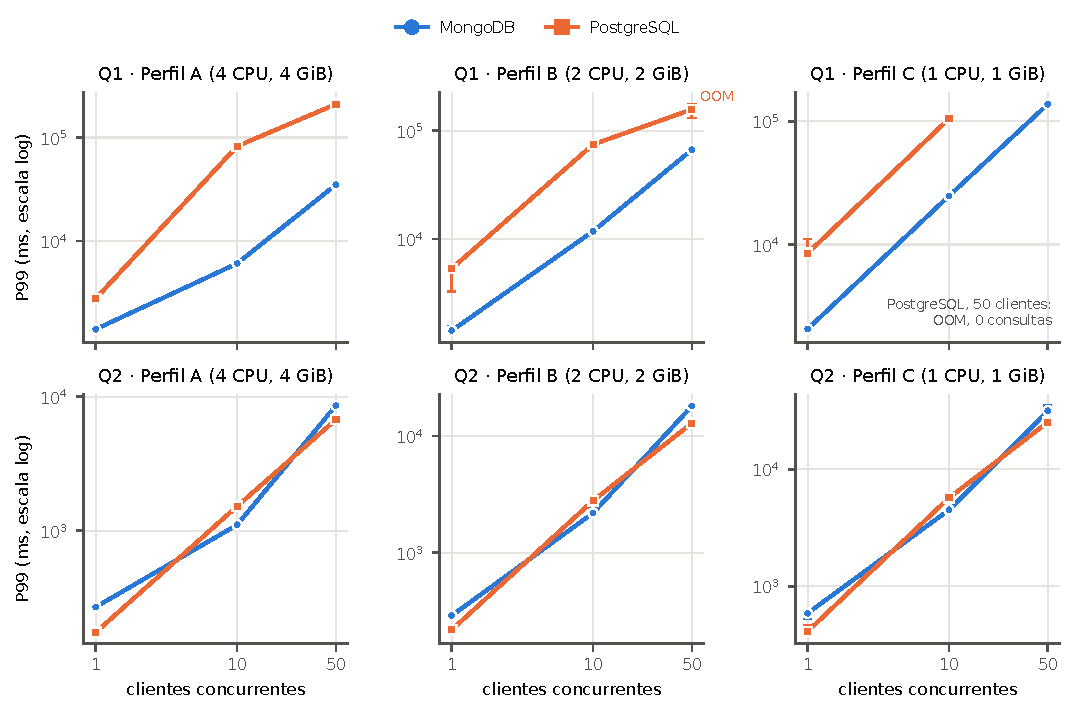
\includegraphics[width=\linewidth]{generado/fig_p99_concurrencia.pdf}
\caption{P99 frente a concurrencia (mediana de 3 rondas; las barras muestran el mínimo
y el máximo entre rondas). Escalas logarítmicas. Todas las corridas de PostgreSQL Q1
volcaron a disco; con 50 clientes, B terminó en OOM y C en OOM sin consultas exitosas.}
\label{fig:p99}
\end{figure}

\paragraph{P99 frente a concurrencia (figura~\ref{fig:p99}).} En Q2 las curvas de los dos
motores casi se superponen y crecen de forma aproximadamente lineal con la concurrencia:
en lazo cerrado, una vez saturada la cuota de CPU, cada cliente adicional se forma en la
cola y la latencia aumenta en proporción. En Q1 la curva de PostgreSQL queda siempre arriba
de la de MongoDB, y la distancia es mayor con 10 clientes que con 1 (13,6 veces en el
perfil A), porque las ejecuciones simultáneas compiten por el mismo disco.

\begin{figure}[h]
\centering
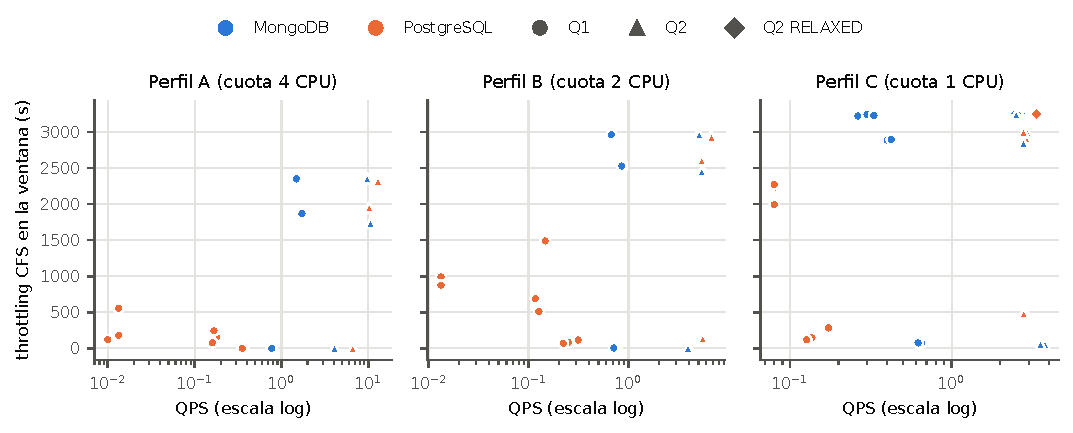
\includegraphics[width=\linewidth]{generado/fig_throttling_qps.pdf}
\caption{Throttling de CFS en la ventana (\cod{throttled\_usec} de \cod{cpu.stat}) frente
a QPS; una marca por corrida (114). Eje de QPS logarítmico.}
\label{fig:throttling}
\end{figure}

\paragraph{Throttling frente a QPS (figura~\ref{fig:throttling}).} Se forman dos grupos.
Con 10 y 50 clientes, las corridas limitadas por CPU (todas las de MongoDB y las de Q2 en
PostgreSQL) tienen throttling en el 100\,\% de los periodos y acumulan entre 1\,700 y
3\,300\,s por ventana, más cuanto menor es la cuota. Su QPS es casi proporcional a la cuota:
Q2 con 50 clientes da 12,93/6,68/3,42\,QPS en PostgreSQL y 9,74/5,09/2,59 en MongoDB
para 4/2/1 CPU (razón cercana a 3,8:2:1). En cambio, PostgreSQL Q1 tiene poco throttling
y además muy bajo QPS: en el perfil A con 10 clientes, solo el 14\,\% de los periodos
tienen throttling. Esa consulta espera al disco, no a la CPU. Con 1 cliente, el
throttling es casi nulo en A y B, pero no en C: MongoDB Q1 tiene throttling en el
63\,\% de los periodos y su P99 sube de 1\,411 a 2\,063\,ms aunque solo haya un cliente.
Como el throttling solo ocurre cuando el grupo agota su cuota dentro de un periodo, esto
indica que, con una sola consulta, MongoDB usa más de una CPU durante parte del tiempo.

\begin{figure}[h]
\centering
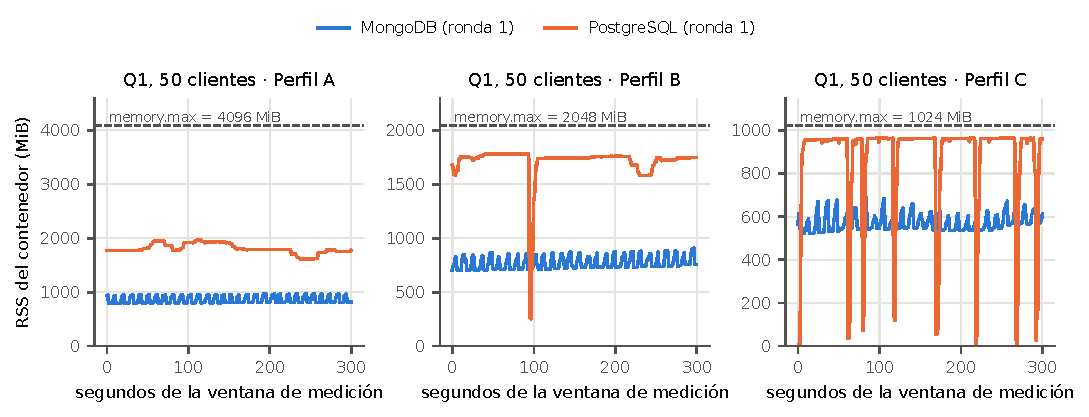
\includegraphics[width=\linewidth]{generado/fig_rss.pdf}
\caption{RSS del contenedor cada segundo (cAdvisor) durante la ventana de medición, Q1
con 50 clientes, ronda 1. La línea discontinua es \cod{memory.max}. Las caídas de
PostgreSQL en B y C son OOM kills: el kernel mata un proceso y PostgreSQL reinicia todos
sus procesos.}
\label{fig:rss}
\end{figure}

\paragraph{Curva RSS (figura~\ref{fig:rss}).} MongoDB se mantiene por debajo de
1\,GiB en los tres perfiles (entre unos 550 y 980\,MiB), con oscilaciones regulares y sin
acercarse al límite. Con 50 clientes en Q1, PostgreSQL ocupa entre 1\,800 y 1\,970\,MiB
de RSS en el perfil A: casi todo el límite de B (2\,048\,MiB) y casi el doble que el de C. En B la RSS
sube hasta cerca de 1\,780\,MiB y cae casi a cero cuando ocurre el OOM kill; en C toca
los 960\,MiB y cae una y otra vez durante toda la ventana.

%=====================================================================
\section{Planes de ejecución}\label{sec:planes}
%=====================================================================
Los planes se guardaron antes de medir, con el perfil A y un solo cliente, usando
\cod{runner/explain\_plans.py}. MongoDB, con \cod{explain} en modo
\cod{executionStats}; PostgreSQL con \cod{EXPLAIN} y las opciones \cod{ANALYZE},
\cod{BUFFERS}, \cod{VERBOSE} y \cod{SETTINGS}.
Están completos en \cod{evidence/plans/}. La tabla~\ref{tab:planes} los pone lado a lado.
Cada valor sale de esos archivos y corresponde a una sola ejecución con el perfil A y 1
cliente: \emph{no} es lo medido en la matriz (secciones 3 y 4).

\begin{table}[h]
\centering\footnotesize
\caption{Planes lado a lado (\texttt{evidence/plans}, perfil A, 1 cliente, una ejecución; no es lo medido en la matriz)}\label{tab:planes}
\begin{tabular}{@{}llp{3.0cm}p{2.0cm}p{2.4cm}p{3.3cm}r@{}}
\toprule
& Motor & Operador principal & Examinados & Ordenamiento o agrupamiento & Memoria o disco & \begin{tabular}[b]{@{}c@{}}Tiempo\\(ms)\end{tabular} \\
\midrule
Q1 & MongoDB & \texttt{COLLSCAN} $\to$ \texttt{\$unwind} $\to$ \texttt{\$group} & 500\,000 docs. & \texttt{\$group}, 90 grupos & memoria: pico 42\,870 B; \texttt{usedDisk}: false & 2\,535 \\
Q1 & PostgreSQL & \texttt{Parallel Seq Scan} $\to$ \texttt{Sort} $\to$ \texttt{Incremental Sort} $\to$ \texttt{Aggregate (Sorted)} & 500\,000 filas & Sort: \texttt{external merge} (3 procesos); Incremental Sort: \texttt{external merge} & disco: Sort 186\,640/199\,600/198\,264 kB; 201\,090 bloques temporales escritos & 3\,838{,}8 \\
\addlinespace
Q2 & MongoDB & \texttt{IXSCAN} (\texttt{fecha\_1}) $\to$ \texttt{FETCH} $\to$ \texttt{SORT} & 227\,094 docs. (193\,203 pasan el filtro) & \texttt{SORT} con límite 1\,000 & memoria: 1\,598\,598 B ordenados, pico 1\,600\,108 B (límite 104\,857\,600 B); \texttt{usedDisk}: false & 266 \\
Q2 & PostgreSQL & \texttt{Parallel Index Scan} (\texttt{ventas\_fecha\_idx}) $\to$ \texttt{Sort} $\to$ \texttt{Gather Merge} $\to$ \texttt{Limit} & 227\,094 filas (193\,203 pasan el filtro) & \texttt{top-N heapsort} & memoria: 3\,071/3\,040/3\,059 kB; 0 bloques temporales & 185{,}1 \\
\bottomrule
\multicolumn{7}{p{0.97\linewidth}}{\scriptsize PostgreSQL: valores de \texttt{EXPLAIN} en JSON; filas examinadas = (filas + filas eliminadas por el filtro) $\times$ loops del nodo de lectura; espacio de ordenamiento del líder y de cada trabajador. MongoDB: \texttt{explain} en modo \texttt{executionStats}. El tiempo es el de esa única ejecución del plan.}\\
\end{tabular}
\end{table}


\paragraph{Q1 en PostgreSQL vuelca a disco.} El planificador ordena los documentos JSONB
completos (\cod{width=1172}) por \cod{tipo\_pago} en un \cod{Sort} paralelo, antes de
desanidar los artículos, para alimentar un \cod{Incremental Sort} y un
\cod{GroupAggregate}. Cada uno de los 3 procesos (líder y 2 trabajadores) ordena
unos 190--200\,MB, muy por encima de \cod{work\_mem} (4\,MB por defecto):

\begin{lstlisting}
GroupAggregate (actual time=1971.048..3137.176 rows=90.00 loops=1)
  Buffers: shared hit=358 read=80006, temp read=200883 written=201096
  ->  Incremental Sort (... rows=674686.00 loops=1)
        Pre-sorted Groups: 3  Sort Method: external merge  Average Disk: 141280kB
        ->  Nested Loop
              ->  Gather Merge  (Workers Launched: 2)
                    ->  Sort  (... rows=166666.67 loops=3)
                          Sort Key: ((ventas.data ->> 'tipo_pago'::text))
                          Sort Method: external merge  Disk: 190536kB
                          Worker 0: Sort Method: external merge  Disk: 202128kB
                          Worker 1: Sort Method: external merge  Disk: 191872kB
                          ->  Parallel Seq Scan on public.ventas
              ->  Function Scan on jsonb_array_elements item (loops=500000)
Execution Time: 3211.518 ms
\end{lstlisting}

\noindent La ejecución del \cod{EXPLAIN} escribió 840\,851\,456 bytes temporales
(\cod{pg\_stat\_database}), unos 0,78\,GiB. En la matriz, el volumen por consulta con 1
cliente es el mismo: 87,7\,GiB para 110 consultas en el perfil A, 60,1\,GiB para 75 en B
y 33,1\,GiB para 41 en C, es decir, unos 0,8\,GiB por ejecución. Subir \cod{work\_mem} a
64\,MB solo en la sesión no elimina el volcado: el plan sigue con \cod{external merge} y
escribe 804\,732\,928 bytes (\cod{postgres\_Q1\_WM64.txt}; esta variante es solo
evidencia y no se midió en la matriz).

\paragraph{Q1 en MongoDB no vuelca.} El plan es \cod{COLLSCAN} sobre los 500\,000
documentos, \cod{\$unwind}, \cod{\$match}, \cod{\$project} y \cod{\$group} con 90 grupos;
\cod{usedDisk: false} y 2\,535\,ms en el perfil A. El \cod{\$group} solo guarda los 90
acumuladores, así que su memoria no depende del tamaño de la colección, y nunca reordena
los documentos.

\paragraph{Q2 en ambos motores.} Los dos usan el índice de \cod{fecha} y un ordenamiento
Top-N en memoria:
\begin{itemize}
\item PostgreSQL: \cod{Parallel Index Scan using ventas\_fecha\_idx}, filtro de
  \cod{es\_fiado} y \cod{Sort Method: top-N heapsort Memory: 3070kB} en cada proceso;
  0 bytes temporales con 4\,MB y con 64\,MB.
\item MongoDB: \cod{IXSCAN} sobre \cod{fecha}, 227\,094 documentos examinados,
  \cod{SORT} con 1\,598\,598 bytes ordenados (el límite por etapa es 104\,857\,600 bytes) y
  \cod{usedDisk: false} con \cod{allowDiskUse} en \cod{false} y en \cod{true}.
\end{itemize}
Como Q2 solo conserva las 1\,000 mejores filas, el ordenamiento nunca llena la memoria
disponible, y las variantes restrictiva y relajada dan el mismo plan. Eso explica que
\cod{Q2\_RELAXED} no cambie las métricas (sección 3). El criterio para medir más celdas
relajadas (fijado antes de medir: que el plan cambiara entre variantes) no se cumplió.

%=====================================================================
\section{Interpretación: límites de memoria, volcado a disco y throttling}
%=====================================================================
\subsection{Respuestas a las preguntas del enunciado (M1, M2, M3)}

\paragraph{M1. ¿Cómo cambian la latencia P95 y P99 de las agregaciones sobre documentos
anidados al limitar CPU y memoria?} En la agregación Q1, MongoDB aumenta su latencia casi
en proporción a la cuota de CPU cuando hay concurrencia: con 10 clientes el P99 pasa de
6\,090 a 11\,808 y 24\,799\,ms (perfiles A, B y C) y el P95 de 5\,923 a 11\,505 y
23\,801\,ms; con 50 clientes el P99 pasa de 35\,077 a 66\,694 y 137\,694\,ms. Con 1 cliente
el cambio es menor (P99 de 1\,411, 1\,429 y 2\,063\,ms). PostgreSQL parte de latencias más
altas por el volcado a disco (P99 con 1 cliente: 2\,790, 5\,343 y 8\,497\,ms; P95: 2\,744,
5\,038 y 8\,179\,ms) y con 50 clientes deja de responder: en B termina en OOM con 4
consultas por ventana y en C en OOM sin ninguna. Con 10 clientes su P99 no sigue a la
cuota (82\,581, 74\,662 y 105\,002\,ms), porque espera al disco. Detalle en la
tabla~\ref{tab:rendimiento} y la figura~\ref{fig:p99} (sección 4).

\paragraph{M2. ¿Qué motor usa de forma más eficiente los buffers de ordenamiento y
agrupamiento antes de volcar a disco o fallar por OOM?} En Q1, MongoDB: su \cod{\$group}
alcanza un pico de 42\,870\,B para 90 grupos y no usa disco (tabla~\ref{tab:planes}), y en
sus 57 corridas no hubo volcado ni OOM (tabla~\ref{tab:recursos}). PostgreSQL ordena los
documentos completos con un \cod{work\_mem} de 4\,MB, vuelca unos 0,8\,GiB por ejecución
en los tres perfiles (21 corridas \cod{spill}) y con 50 clientes falla por OOM en B y C
(6 corridas). En Q2 no hay diferencia: los dos resuelven el Top-1000 en memoria (unos
3\,MB en PostgreSQL y 1,6\,MB en MongoDB) sin volcar, con ambas variantes de memoria
(sección~\ref{sec:planes}).

\paragraph{M3. ¿Cuál es la huella de CPU y memoria por cada 1\,000 documentos procesados en
cada motor?} Con la definición adoptada en la sección 3 (el enunciado no la precisa), en Q1
con 1 cliente PostgreSQL
usa 8,7--11,8\,ms de CPU por cada 1\,000 documentos y MongoDB 2,9--3,2\,ms; en Q2 los dos
quedan entre 1,1 y 1,8\,ms (tabla~\ref{tab:huella}). En memoria, MongoDB mantiene una RSS
mediana de 493 a 974\,MiB y PostgreSQL usa menos RSS en Q2 (mediana de 20 a 298\,MiB), con la salvedad sobre
la memoria compartida que se indica en la sección 3. Las celdas de PostgreSQL Q1 con 50
clientes no tienen una huella comparable (pocas consultas u OOM).

\subsection{Análisis}

\paragraph{El cuello de botella de PostgreSQL Q1 es el plan, no el límite de memoria.} El
volcado aparece desde el perfil A con 1 cliente (4\,GiB de límite y 0,1\,\% de periodos
con throttling) y con el mismo volumen, unos 0,8\,GiB por ejecución, en los tres perfiles.
Lo que lo provoca es la decisión del planificador de ordenar los documentos completos
antes de desanidarlos, con un \cod{work\_mem} de 4\,MB por nodo de ordenamiento; el límite
del contenedor no interviene. Por eso su throttling es bajo y su QPS cae con la
concurrencia: con 10 clientes en A el QPS baja de 0,37 a 0,17, aunque haya CPU libre
(86\,\% de los periodos sin throttling). Las consultas se forman detrás del disco.

\paragraph{El OOM aparece cuando la memoria de 50 sesiones no cabe en el límite.} En el
perfil A, 50 clientes de Q1 llevan la RSS de PostgreSQL a 1\,970\,MiB y
\cod{memory.peak} llega a los 4\,096\,MiB del límite; no hay OOM porque esa diferencia es
caché de página de los archivos temporales, que el kernel puede liberar. En B el límite es
de 2\,048\,MiB: la RSS sube a unos 1\,780\,MiB y, sumada a la caché de los temporales,
toca el límite; sin swap (\cod{memory.swap.max = 0}), el kernel mata un proceso
(5 OOM kills en 3 rondas). En C (1\,024\,MiB) la RSS llega a 960\,MiB en segundos y hay
144 OOM kills en 3 rondas. En los registros de PostgreSQL se ve
\cod{client backend \ldots was terminated by signal 9: Killed} seguido de
\cod{all server processes terminated; reinitializing} y de una recuperación automática:
cada OOM kill tira todas las sesiones, no solo la que lo provocó, y por eso hay errores
de conexión (12\,168 en C y 428 en B). \emph{Hipótesis no verificada:} la RSS por sesión
viene de los búferes de ordenamiento de hasta 3 procesos por consulta y de la compilación
JIT que muestra el plan (191\,ms de JIT por ejecución).

\paragraph{MongoDB se degrada por CPU, no por memoria.} MongoDB no volcó a disco ni tuvo
OOM; su RSS se mantuvo por debajo de 1\,GiB en todos los perfiles. En Q1 su QPS con 10
clientes es casi proporcional a la cuota de CPU (1,72/0,87/0,42 para 4/2/1 CPU), y su P99
con 50 clientes crece en la misma proporción (35, 67 y 138\,s). En el perfil C su
\cod{memory.peak} llega a 1\,024\,MiB con Q1 y 50 clientes sin OOM: la memoria que
excede la RSS es caché que el kernel recupera.

\paragraph{El throttling mide saturación de la cuota, no trabajo perdido.} Con 10 o más
clientes, toda corrida limitada por CPU tiene throttling en el 100\,\% de los periodos, y
los segundos acumulados crecen al bajar la cuota (por ejemplo, Q2 con 50 clientes en
PostgreSQL: 2\,322, 2\,935 y 3\,237\,s en A, B y C). Como el contador suma el tiempo de
espera de todas las CPU, sirve para comparar celdas y para ver cuándo la cuota está
saturada, pero no se puede leer como ``segundos de reloj perdidos''. El indicador que
traduce el throttling al usuario es el QPS, que en esas corridas escala con la cuota.

\paragraph{Q2: con un Top-1000 no hay presión de memoria.} Ninguna variante vuelca a disco
porque el ordenamiento Top-N solo conserva 1\,000 filas (unos 3\,MB en PostgreSQL y
1,6\,MB en MongoDB). La diferencia entre motores en Q2 es de CPU: PostgreSQL usa
trabajadores paralelos y responde antes con 1 cliente; con 50 clientes saca unas 1,3 veces más
QPS con la misma cuota (1,33, 1,31 y 1,32 en A, B y C). \emph{Hipótesis no verificada:} el costo por
consulta de PostgreSQL en Q2 es menor porque lee los documentos JSONB desde el índice y
descarta pronto los que no entran en el Top-N.

%=====================================================================
\section{Recomendaciones técnicas}
%=====================================================================
Para el sistema de abarrotes, a partir de lo medido:
\begin{enumerate}
\item \textbf{Agregaciones sobre los artículos de las ventas (tipo Q1).} Con el esquema
  JSONB tal como está, no conviene ejecutarlas en PostgreSQL de forma concurrente: cada
  ejecución escribe unos 0,8\,GiB temporales y con 50 clientes provocó OOM con 1 y 2\,GiB.
  Las opciones, en orden de esfuerzo:
  \begin{itemize}
  \item Ejecutarlas en MongoDB, que las resolvió sin disco y sin OOM en todos los perfiles.
  \item En PostgreSQL, guardar los artículos en una tabla relacional (o en una columna
    generada) para no ordenar el documento JSONB completo. \emph{No se midió.}
  \item Limitar la concurrencia de estos reportes (por ejemplo, una cola o un
    \textit{pool} de 1 a 2 conexiones), porque el volumen temporal crece con los clientes.
  \end{itemize}
\item \textbf{No confiar en subir \cod{work\_mem}.} Con 64\,MB el plan de Q1 sigue
  volcando; además, \cod{work\_mem} se reserva por nodo y por proceso, y con muchas
  sesiones el riesgo de OOM aumenta. Cualquier cambio debe probarse con el
  \cod{EXPLAIN} y con la concurrencia real.
\item \textbf{Dimensionar la memoria de PostgreSQL por sesión, no por consulta.} Con 50
  sesiones de Q1, la RSS llegó a unos 2\,GiB; un contenedor de 1--2\,GiB no basta. Con
  límites estrictos, conviene un \textit{pooler} que limite las conexiones activas.
\item \textbf{Consultas de listado tipo Q2.} Ambos motores las resuelven en memoria; si el
  objetivo es la latencia con pocos clientes, PostgreSQL fue más rápido. Para más
  clientes, lo que importa es la cuota de CPU: el QPS escaló casi en proporción a ella.
  Las variantes de memoria (\cod{allowDiskUse}, \cod{work\_mem}) no aportan nada aquí.
\item \textbf{Vigilar el throttling junto con el QPS.} En producción, un 100\,\% de
  periodos con throttling indica que la cuota de CPU está saturada; si coincide con un QPS
  que no sube, hace falta más CPU. Un QPS bajo con poco throttling, como PostgreSQL Q1,
  apunta al disco o al plan.
\end{enumerate}
\textbf{Trabajo futuro (no medido):} esquema relacional de los artículos en PostgreSQL,
efecto de desactivar JIT o el paralelismo en Q1, índices sobre \cod{total} para Q2, y
repetir la matriz en Linux nativo.

%=====================================================================
\section*{Desviaciones y limitaciones}\label{sec:desviaciones}
\addcontentsline{toc}{section}{Desviaciones y limitaciones}
%=====================================================================
\begin{enumerate}
\item \textbf{Entorno.} Docker Desktop sobre WSL2 en Windows, no Linux nativo. La VM tiene
  12 CPU y 7,39\,GiB; el cliente de carga corre en Windows y comparte el procesador con la
  VM.
\item \textbf{Dataset adaptado al proyecto de abarrotes.} En lugar de las órdenes del
  enunciado: \cod{es\_fiado = false} reemplaza al estado \cod{completed}; \cod{tipo\_pago}
  a país; el proveedor del artículo a categoría; \cod{folio} desempata el orden de Q2; el
  \cod{id} de PostgreSQL es un UUID determinista (uuid5) calculado del \cod{\_id}. Cada
  artículo lleva un subdocumento \cod{producto} para llegar a 4 niveles. Datos
  sintéticos; 940\,B por venta en JSON.
\item \textbf{Tolerancia en Q1.} Las sumas de MongoDB son \cod{double} y las de
  PostgreSQL \cod{numeric}; se aceptó una diferencia de hasta 1 centavo (la máxima fue
  $9{,}3\times10^{-10}$).
\item \textbf{\cod{shm\_size: 1g} en PostgreSQL.} El \cod{/dev/shm} de 64\,MB que Docker
  da por defecto corta las consultas paralelas. Es un ajuste de Docker, no del motor.
\item \textbf{Swap.} \cod{mem\_swappiness: 0} no se aplica en cgroups v2 (Docker lo
  ignora); el swap se anuló con \cod{memswap\_limit} igual a la memoria y se verificó
  \cod{memory.swap.max = 0}.
\item \textbf{Puerto de MongoDB.} El contenedor se publica en el 27018 porque el 27017 lo
  usa un servicio MongoDB de Windows, que se mantuvo detenido durante la matriz.
\item \textbf{Throttling.} El valor del CSV sale de \cod{cpu.stat} y suma todas las CPU,
  por lo que puede superar los 300\,s de la ventana. La serie de cada segundo de cAdvisor
  tiene una resolución efectiva de unos 2\,s.
\item \textbf{Percentiles con pocas consultas.} En PostgreSQL Q1 con 50 clientes
  terminan 3 o 4 consultas por ventana (perfiles A y B): su P95 y su P99 son el máximo.
  Varias celdas de Q1 tienen menos de 100 consultas (marcadas con $\dagger$).
\item \textbf{Temporales tras un OOM.} PostgreSQL reinicia sus estadísticas al
  recuperarse de un OOM kill, así que en las corridas \cod{oom} los bytes temporales no
  se pudieron medir: \cod{disk\_spill} queda vacío y nunca se estima.
\item \textbf{Serie de RSS de cada segundo.} El runner consultó cAdvisor por nombre de
  contenedor y tomó la primera serie devuelta; cuando el contenedor se recrea, Prometheus
  conserva unos minutos la serie del contenedor anterior con el mismo nombre. Una
  auditoría posterior (\cod{analysis/auditar\_rss.py}), que filtra por el id del
  contenedor de cada corrida, encontró que en 24 de las 114 corridas el
  \cod{serie\_1s.csv} guardado es de otro contenedor; la figura~\ref{fig:rss} usa las
  series corregidas (\cod{report/generado/rss\_corregida/}). El \cod{max\_rss\_mb} del
  CSV es correcto en las 114 corridas, y el throttling del CSV sale del cgroup, así que
  no se ve afectado.
\item \textbf{Piloto.} En el CSV del piloto (\cod{results/piloto/}, fuera de la matriz)
  la fila de PostgreSQL C Q1 con 50 clientes, que terminó en \cod{oom}, quedó con
  \cod{disk\_spill = false} sin haberse medido. Se corrigió el runner antes de la matriz y
  el CSV del piloto se conserva tal como salió.
\item \textbf{Lazo cerrado.} Los clientes lanzan la siguiente consulta en cuanto termina
  la anterior, sin tiempo de espera; con 50 clientes la latencia refleja sobre todo la
  cola, no la velocidad de una consulta aislada.
\item \textbf{Pausa.} La matriz se pausó una vez entre corridas (11:59 a 12:49). No hubo
  corridas a medias ni descartes.
\item \textbf{\cod{memory.peak}.} Es el pico del cgroup desde que arranca el contenedor,
  incluido el calentamiento, y cuenta caché de página; no equivale a la RSS.
\item \textbf{Huella por cada 1\,000 documentos (M3).} Es una definición adoptada en este
  reporte, porque el enunciado no la precisa. El CPU
  de la ventana incluye el de las consultas en vuelo que se cancelan al cerrarla, lo que
  sesga la huella hacia arriba, sobre todo con pocas consultas ok, y no incluye el
  cliente, que corre en Windows. Los documentos por consulta salen de los planes con el
  perfil A y 1 cliente y se asumen constantes. La razón de RSS por documentos/s es una
  interpretación del enunciado.
\item \textbf{Variante relajada en el CSV.} Las 6 filas de \cod{Q2\_RELAXED} (2 celdas
  $\times$ 3 rondas) usan \cod{query\_id = Q2\_RELAXED}, valor que el esquema del
  enunciado no define; se usó para reportar ambas variantes de Q2 sin agregar ni renombrar
  columnas. Para concatenar con otros CSV conviene filtrarlas o tratarlas como Q2.
\end{enumerate}

%=====================================================================
\appendix
\section{Reproducción y archivos}
%=====================================================================
Desde la raíz del repositorio, con el entorno de Python de \cod{requirements.txt}:
\begin{lstlisting}
docker compose --profile telemetry up -d       # Prometheus, cAdvisor y Node Exporter
python synthetic_data_generator.py              # 500 000 ventas, semilla 20261101
python runner/load_data.py                      # carga e índices en ambos motores
python runner/verificar_f2.py                   # verificación del baseline
python runner/explain_plans.py --out evidence/plans --queries Q1 Q1_WM64 Q2 Q2_RELAXED
./run_benchmarks.sh --rondas 3 --timeout 300    # matriz completa (orquestador)
python analysis/auditar_rss.py                  # auditoría de la RSS (con Prometheus)
python analysis/consolidar.py                   # tablas y figuras de este reporte
\end{lstlisting}

\begin{itemize}
\item \cod{results/benchmark\_results.csv}: las 114 filas (14 columnas fijas).
\item \cod{results/ronda\_0n/runs/<run\_id>/}: \cod{meta.json}, \cod{latencias.csv},
  \cod{serie\_1s.csv} y, en \cod{oom}, \cod{docker\_logs.txt}.
\item \cod{results/bitacora.log}: eventos con hora (inicio, pausa, reanudación, respaldos).
\item \cod{evidence/INDEX.md}: una línea por cada corrida \cod{spill} u \cod{oom} con sus
  archivos.
\item \cod{evidence/plans/}, \cod{evidence/verificacion/}, \cod{evidence/entorno/}.
\end{itemize}

El manifiesto de la ronda 3 (el final) verifica con \cod{sha256sum -c} en un clon del
repositorio, salvo cuatro archivos que el orquestador actualizó después de hacer ese
respaldo: \cod{bitacora.log}, \cod{estado.txt}, \cod{resumen.md} y
\cod{orquestador\_matriz.out}. Los manifiestos de las rondas 1 y 2 son copias intermedias:
además de esos archivos difieren \cod{benchmark\_results.csv} y \cod{evidence/INDEX.md},
que siguieron creciendo después de cada respaldo.

\end{document}
